\documentclass[12pt]{article}  % [12pt] option for the benefit of aging markers
\usepackage{amssymb,amsthm}    % amssymb package contains more mathematical symbols
\usepackage{graphicx}          % graphicx package enables you to paste in graphics

\usepackage{tabularx}
\usepackage{setspace}
\usepackage[nottoc,notlot,notlof]{tocbibind}

%%%%%%%%%%%%%%%%%%%%%%%%%%%%%%%%%
%
%    Page size commands.  Don't worry about these
%
\setlength{\textheight}{220mm}
\setlength{\topmargin}{-10mm}
\setlength{\textwidth}{150mm}
\setlength{\oddsidemargin}{0mm}

%%%%%%%%%%%%%%%%%%%%%%%%%%%%%%%%%%%%%%%%%%%%%%%%%%%%%%%%%%%%%%%
%
%    Definitions of environments for theorems etc.
%
\newtheorem{theorem}{Theorem}[section]          % Theorems numbered within sections - eg Theorem 2.1 in Section 2.
\newtheorem{corollary}[theorem]{Corollary}      % Corollaries etc. will be counted as Theorems for numbering
\newtheorem{lemma}[theorem]{Lemma}              % eg Lemma 3.1, ... Theorem 3.2, ... Corollary 3.3.
\newtheorem{proposition}[theorem]{Proposition}
\newtheorem{conjecture}[theorem]{Conjecture}

\theoremstyle{definition}
\newtheorem{definition}[theorem]{Definition}

\theoremstyle{remark}
\newtheorem{remark}[theorem]{Remark}
\newtheorem{example}[theorem]{Example} 

%%%%%%%%%%%%%%%%%%%%%%%%%%%%%%%%%%%%%%%%%%%%%%%
%
%        Preamble material specific to your essay
%
\title{Lab Marking system \\~\\  \large{Heriot-Watt University} \\~\\ Final Year Dissertation}
\author{Lewis McNeill\\
supervised by
Peter J King}

\begin{document}
\maketitle
\pagenumbering{gobble}
\newpage 

\doublespacing
\textbf{\Large{Declaration}} \\[2em]
I, Lewis Francis McNeill, confirm that this work submitted for assessment is my own and is expressed in my own words. Any uses made within it of the works of other authors in any for (e.g., ideas, equations, figures, text, tables, programs) are properly acknowledged at any point of their use. A list of the references employed is included.
\\
\\
Signed: Lewis McNeill
\\
Date: \today

\newpage                    
\begin{abstract}

The project aim is to develop a web application that will be used to improve marking of computing labs. The application will be designed to be used by Students to quickly know their grade, by Lab Helpers to easily mark labs and Lecturers to see marking immedatly as it is done.



\end{abstract}

\newpage                     

\singlespacing
\tableofcontents
\doublespacing



\newpage        

\section{Aims, Objectives and Project Description}
\setcounter{page}{1}
\pagenumbering{arabic}

\subsection{Aim}
The aim of this dissertation is to design and implement a system for the digital marking and analysis of computer labs, to help improve the speed at which they are marked


\subsection{Objectives}
\begin{itemize}
\item Simplify the way that labs marks are currently processed.
\item Allow lecturers to create marking schemes on-line that lab helps can access and mark students against in labs.
\item Develop a system that allows lab helps to mark labs using an on-line application.
\item Allow students to see the mark they got from the lab instantly.
\item Provide useful statistics and graphs to lecturers.
\end{itemize}






\newpage
\section{Literature Review}

This section contains the current academic literature relating to the digitalisation of marking systems. 
\subsection{Digital Marking Systems}
Digital marking systems are designed to mirror current paper based marking systems but take advantage of the electronic enviroment \cite{EssayType} 

\subsection{User Dependant Views}


\subsection{Data to Graphics}

\newpage
\section{Requirements}
\subsection{System Requirements}


\begin{tabularx}{\textwidth}{|l|X|X|X|X|}
\hline
  \textbf{ID} & \textbf{Requirement} & \textbf{Type} & \textbf{Description} & \textbf{Priority} 
\\
\hline
R1&Test&Test&Test&Test\\ \hline
R2&Test&Test&Test&Test\\ \hline


\end{tabularx}

\subsection{Usability Requirements}


\newpage
\section{Strategy for testing and evaluation}

\subsection{Testing}
Throughout the development of the system, unit tests will be used to make sure that the system is robust and functional. \\

\subsection{Evaluating}
To properly evaluate how successful I have been at creating a new Lab Marking System I will conduct a usability case study. Lecturers, lab helpers and students will be asked to use the systems and provide feed back, to help evaluate the system and discover what improvements can be made to make it better.


\newpage
\section{Project Plan and Professional, Legal, Ethical and Social Issues}

\subsection{Project Plan}

The plan for this dissertation can be seen in figure(\ref{fig:ganttchart})

\begin{figure}[!htbp]

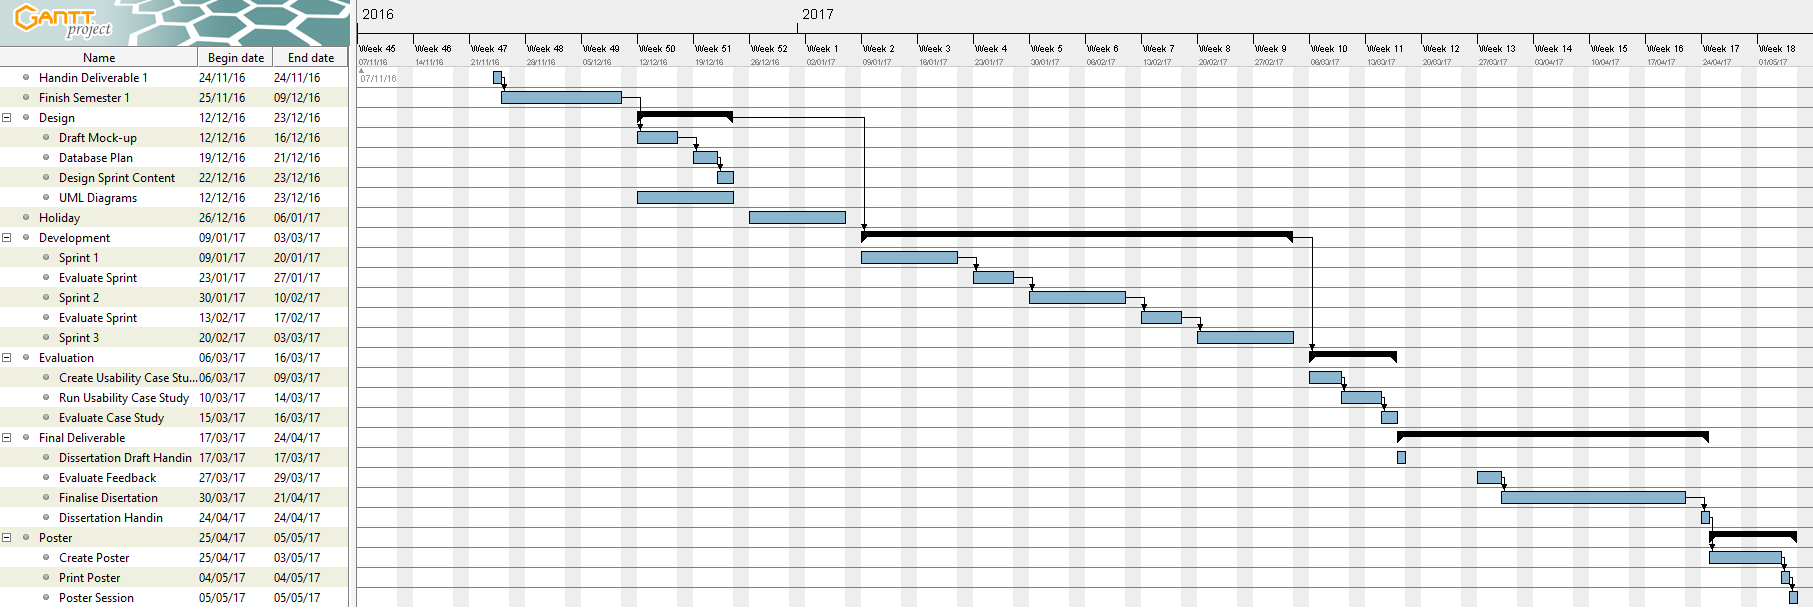
\includegraphics[width=\textwidth]{images/ganttchart.png}
\caption{Project Gantt Chart}
\label{fig:ganttchart}

\end{figure}

\subsection{Risk Analysis}
\newcounter{risk} \stepcounter{risk}

\begin{tabularx}{\textwidth}{|l|X|X|X|}

\hline
  \textbf{ID} & \textbf{Risk} & \textbf{Importance} & \textbf{Likelihood }
\\
\hline
R\arabic{risk} &Test&Test&Test\\ \hline \stepcounter{risk}
R\arabic{risk} &Test&Test&Test\\ \hline \stepcounter{risk}
R\arabic{risk} &Test&Test&Test\\ \hline \stepcounter{risk}
R\arabic{risk} &Test&Test&Test\\ \hline \stepcounter{risk}
R\arabic{risk} &Test&Test&Test\\ \hline \stepcounter{risk}


\end{tabularx}

\subsection{Professional}

\subsection{Legal}
Their are multiple legal issues relating to this project. The most important one is the Data Protection Act, since the systems will be designed to store data about student I will have to make sure that 

\subsection{Ethical}

\subsection{Social}






%%%%%%%%%%%%%%%%%%%%%%%%%%%%%%%%%%%%%%%%%
%
%     Bibliography
%

\newpage


\begin{thebibliography}{99}

% 
% The usual convention for mathematical bibliographies is to list alphabetically
% by first-named author (then second, third  etc. author then date)
% websites with no author names should go by the site name
%



% Typical layout for reference to a journal article
%

\bibitem{EssayType}
E. Heinrich, Y. Wang,
{\em Online Marking of Essay-type Assignments};
2003.(http://www-ist.massey.ac.nz/MarkTool/Publications/EdMedia2003Onscreen.pdf)

\bibitem{Bovey}
J. D. Bovey, M. M. Dodson,                         % author(s)
The Hausdorff dimension of systems of linear forms % article name
{\em Acta Arithmetica}                             % journal name - italics
{\bf 45}                                           % volume number - bold
(1986), 337--358.                                   % (year), page range

% Typical layout for reference to a book
%
\bibitem{Cassels}
J. W. S. Cassels,                                  % author(s)
{\em An Introduction to Diophantine Approximation},% title - italics
Cambridge University Press, Cambridge, 1965.       % Publisher, place, date.

% Typical layout for reference to a website
%
\bibitem{GAP}
The GAP Group, GAP -- Groups, Algorithms, and Programming,  % Site name
Version 4.5.6; 2012. % other information
(http://www.gap-system.org)  % URL


% Typical layout for reference to an online article
%
\bibitem{Howie}
J. Howie,                                            % author(s)
{\em Generalised triangle groups of type $(3,5,2)$}, % article name - italics
http://arxiv.org/abs/1102.2073                       % URL
(2011).                                              % (year)
\end{thebibliography}
\end{document}


